\section{Benchmarking Setup}
\label{setup}

Suppose that there are $S$ simulators, indexed by $s$. The exact order 
of these simulators does not matter, however a consistent ordering should
be used. In the demonstration here, there are two simulators with $s=0$
being DYMOND and Cyclus $s=1$.

Furthermore, for any feature or metric there may be $I$ components, 
indexed by $i$. In this paper, we will look at the power generation feature
that has constituent components of the power generated by LWRs ($i=0$) and
the power generated by FRs ($i=1$).  Again, the ordering of these is not 
important, only that the ordering is consistent. An alternative example
that will not be examined here is the mass flow, which may be partitioned 
by its individual nuclides or by chemical element.

Now, denote a metric for a given simulator and component as 
$m_s^i(t)$, which is a function of time $t$. For many metrics of interest 
to nuclear fuel cycle analysis, the following equality holds:
\begin{equation}
m_s(t) = \sum_i^I m_s^i(t)
\end{equation}
Thus $m_s(t)$ is the total metric over all constituent parts for a given 
simulator. This linear combination is useful when calculating contributions
(\S \ref{contribution}) but is not needed to compare various simulators
to a Gaussian process model (\S \ref{dtw}).

Additionally, call $u_s^i(t)$ the uncertainty or error in the metric 
$m_s^i(t)$. Note that $u$ is also a time series for each simulation for 
each component. If uncertainties are not known, this can be set to floating
point precision (which states that the metric is as precise as possible) or
some nominal fraction of the value (10\%, 20\%, etc). It is, of course, 
much preferred for the simulator and/pr metric evaluator to compute 
uncertainties directly. However, this is often not supported in the underlying
simulator, so in practice another strategy is needed.  

The demonstration here will use the generated power from LWRs and FRs in 
transition scenario covering 200 years. The simulation should start with
90 GWe generated solely by LWRs and meet a 1\% growth in demand over the 
lifetime of the simulation. Figure \ref{gwe-simulators} shows the component time 
series curves for both DYMOND and Cyclus.

\begin{figure}[htb]
\centering
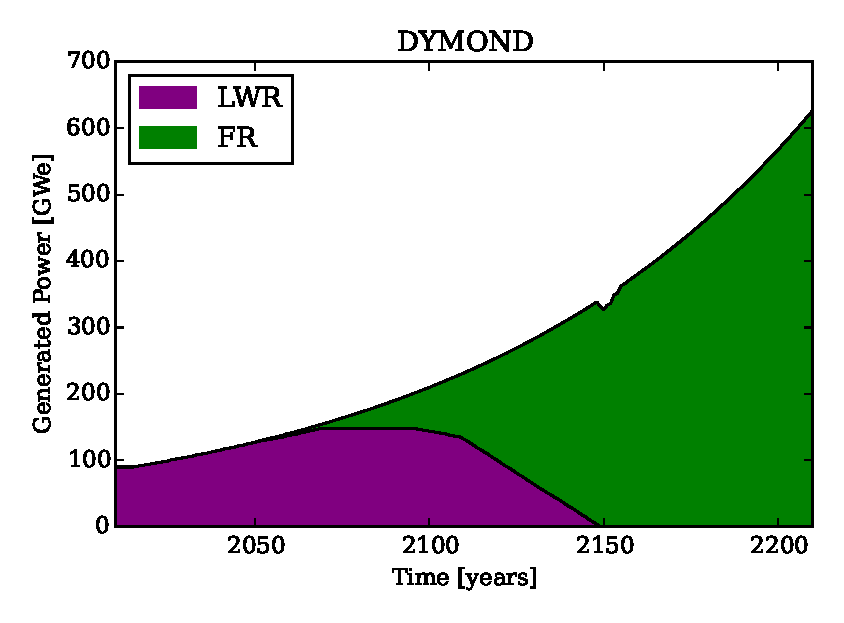
\includegraphics[width=0.45\textwidth]{gwe-dymond.eps}
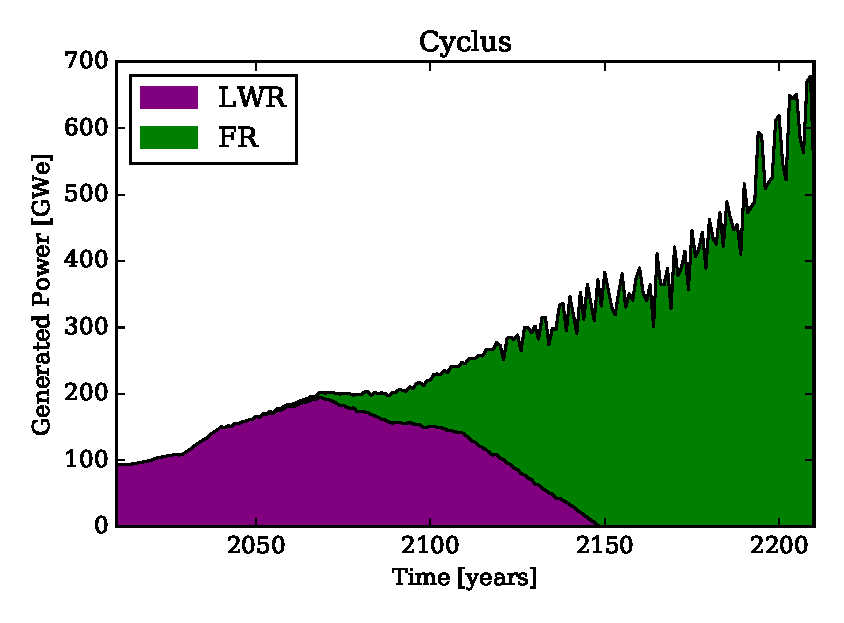
\includegraphics[width=0.45\textwidth]{gwe-cyclus.eps}
\caption{The generated power in [GWe] as a function of time for the DYMOND and 
Cyclus simulators for both LWRs and FRs.}
\label{gwe-simulators}
\end{figure}

\clearpage
